\documentclass[a4paper, 12pt, twoside, openright]{book}
\usepackage[italian]{babel}
\usepackage[T1]{fontenc}
\usepackage[utf8]{inputenc}
\usepackage{fancyhdr}
\usepackage{float}
\usepackage{graphicx}
\usepackage{wrapfig}
\usepackage{setspace}

%------------------------------ colors
\usepackage[usenames,dvipsnames,table]{xcolor} % use colors on table and more
\definecolor{333}{RGB}{51, 51, 51} % define custom color
%------------------------------ source code
\usepackage{listings}
\lstset{
  basicstyle=\footnotesize\sffamily,
  commentstyle=\itshape\color{gray},
  captionpos=b,
  frame=shadowbox,
  language=HTML,
  rulesepcolor=\color{333},
  tabsize=2
}
%------------------------------ define Abstract environment, missing in the 'book' class
\newenvironment{abstract}{\cleardoublepage \null \vfill \begin{center}\bfseries\abstractname \end{center}}{\vfill\null}
\addto\captionsenglish{\renewcommand*\abstractname{Sommario}} % change Abstract title
%------------------------------ active url
\usepackage{url}
\renewcommand{\UrlFont}{\color{black}\small\ttfamily}
\usepackage[colorlinks=true, linkcolor=black, citecolor=black, urlcolor=black]{hyperref} % active ref
%------------------------------ macros
\newcommand{\sectionname}{Section} % define Section ref
\newcommand{\subsectionname}{Sub-section} % define Sub-section ref
\renewcommand*\arraystretch{1.4} % tables padding


\begin{document}
\frontmatter
\begin{titlepage}
	%immagini di intestazione
	\begin{flushleft}
		
		\begin{minipage}[b][1,8 cm][c]{0.3\columnwidth}
			\textsf{{\color{Sepia}{DIPARTIMENTO\\DI INGEGNERIA\\DELL'INFORMAZIONE}}}
		\end{minipage}
	\end{flushleft}
	
	%titoli vari
	\vfill
	\begin{center}
		\begin{large}
			DIPARTIMENTO DI INGEGNERIA DELL'INFORMAZIONE
			\\~\\
			CORSO DI LAUREA IN INGEGNERIA INFORMATICA
			\\~\\~\\
			TITOLO
		\end{large}
	\end{center}
\end{titlepage}
\cleardoublepage % make left page blank

\begingroup %------------------------------ CONTENTS
  \makeatletter
  \let\ps@plain\ps@empty
  \makeatother
  \tableofcontents
  \clearpage
\endgroup


\begin{abstract} %------------------------------ ABSTRACT
\markboth{}{} % remove header
\thispagestyle{empty}
\end{abstract}


\mainmatter\doublespace 

\chapter*{Introduzione} %------------------------------ INTRODUCTION
\thispagestyle{empty}

\chapter{Strumenti Web utilizzati nelle PWA}
%SERVONO ESEMPI?
Questa sezione copre le tecnologie web usate nelle Web App che non sono vincolate a uno specifico framework di sviluppo: di esse si fornirà una descrizione delle relative funzionalità e di una loro possibile implementazione in JavaScript.\\
Alcuni screenshot di questa sezione sono stati catturati dai Developer Tools (DevTools) del browser: per visualizzarli su PC è sufficiente premere F12 (valido per Firefox e per qualunque browser Chromium-based come Google Chrome o Microsoft Edge). Le immagini fanno in particolare riferimento ai DevTools di Google Chrome.

\section{Cookie}
Un \textit{Cookie} è una stringa di testo che viene inviata dal server web al client, il quale avrà poi il compito di memorizzarla e reinviarla al server, senza modifiche, ogni volta che accede alla stessa porzione di uno stesso dominio web \cite{Wiki:cookies}.\\
I Cookie hanno una dimensione ridotta: infatti, dato che il browser può dover inoltrare anche centinaia di Cookie durante la navigazione, delle dimensioni eccessive provocherebbero danni alle prestazioni. Essi sono inviati attraverso specifici header del protocollo \textit{HTTP}: nel caso di \textit{HTTP response} viene usato l'header \texttt{Set-Cookie} mentre per la \textit{HTTP request} si usa \texttt{Cookie} \cite{Wiki:cookies}. A un Cookie viene associata inoltre una data di scadenza, oltre la quale non viene considerato più valido \cite{Wiki:cookies}.\\
I Cookie possono avere diversi scopi: possono coprire funzionalità necessarie al corretto funzionamento del sito (in tal caso si parla di \textit{cookie tecnici}), possono raccogliere dati in forma anonima a fini statistici (\textit{cookie statistici}) oppure possono tracciare la navigazione dell'utente, con lo scopo di costruire un profilo personalizzato del cliente utile a fornire annunci mirati (\textit{cookie pubblicitari}) \cite{Wiki:cookies}. Questi ultimi sono stati oggetto di diverse discussioni, in quanto un loro abuso potrebbe costituire una minaccia alla privacy degli utenti; per questo motivo il loro utilizzo è normato da svariate leggi in diversi stati: in Europa il \textit{GDPR} (\textit{General Data Protectioni Regulation}) ha stabilito che tutti i siti internet che fanno uso di Cookie pubblicitari di terze parti sono obbligati a comunicarlo all'utente all'inizio della sua navigazione nella pagina web \cite{Cookiebot}. Tale comunicazione deve essere effettuata attraverso un banner che ostacoli la visualizzazione della pagina: in esso devono essere elencati tutti i Cookie pubblicitari presenti nel sito, specificando anche chi elaborerà i dati raccolti e con quali finalità \cite{Cookiebot}; è inoltre obbligatorio fornire la possibilità di negare il consenso dei singoli Cookie, non è sufficiente permettere all'utente di negare/consentire tutti i Cookie in blocco \cite{Cookiebot}. Un Cookie non potrà essere attivato se non dopo il consenso esplicito da parte dell'utente, il quale sarà registrato in opportuna documantazione a testimoniare alle autorità che l'autorizzazione è stata concessa \cite{Cookiebot}. Il consenso a un Cookie deve essere fornito mediante un'azione non equivoca (come ad esempio cliccare sul pulsante "Acconsento"); azioni come continuare la navigazione sul sito non devono essere considerate come permesso per installare i Cookie \cite{Cookiebot}. Si deve inoltre fornire la possibilità di modificare le proprie scelte in un secondo momento. All'inizio della navigazione tutti i Cookie di terze parti e non strettamente necessari al corretto funzionamento del servizio devono essere preventivamente disattivati in attesa della scelta dell'utente. Una volta confermata la scelta il \textit{Cookie di consenso} si occuperà di attivare tutti i soli Cookie inserzionistici per il quale l'utente ha dato esplicito consenso \cite{Cookiebot}.\\
Diversi siti internet fanno uso dei cookie come identificatore di sessione univoco dell'utente (utile ad esempio per permettere al cliente di mantenere l'accesso senza dover fare continuamente login): questo può costituire un rischio per la sicurezza, in quanto un utente malintenzionato può rubare il cookie di qualcun altro e sfruttarlo per impersonare la vittima. Questo problema può essere risolto sfruttando soli Cookie con la flag "\texttt{Secure}" (che consente l'invio del Cookie solo attraverso protocollo criptato HTTPS) \cite{Wiki:cookies}.
\subsection{implementazione}
I Cookie hanno un'interfaccia molto primitiva: non sono definite, infatti, delle funzioni per l'aggiunta, rimozione o la modifica di essi. L'unico modo per inserire, modificare, leggere ed eliminare Cookie è mediante l'attributo \texttt{document.cookie} \cite{MDN_Web_docs:cookies}.\\
Per inserire un nuovo Cookie basta assegnare una nuova stringa a \linebreak\texttt{document.cookie} \cite{MDN_Web_docs:cookies}: tale stringa dovrà presentarsi nel formato \linebreak\texttt{"name=value; optionalField1=optionalValue1; optionalField2=\linebreak optionalValue2;..."} \cite{MDN_Web_docs:cookies}. La coppia \texttt{"name=value"} deve essere specificata, altrimenti l'inserimento fallirà silenziosamente, tutte le coppie successive sono invece opzionali. I campi opzionali sono i seguenti:
\begin{itemize}
\item\texttt{"expires="}: definisce la data di scadenza del Cookie come stringa UTC; per esprimere una data in tale formato è possibile usare il metodo \texttt{toUTCString()} della classe \texttt{Date} definita in JavaScript \cite{MDN_Web_docs:cookies}. Se non sono specificati né \texttt{expires} né \texttt{max-age} allora il Cookie scadrà al termine della sessione \cite{MDN_Web_docs:cookies}.
\item\texttt{"max-age="}: specifica la durata del Cookie in secondi \cite{MDN_Web_docs:cookies}.
\item\texttt{"secure"}: indica che il Cookie può essere trasmesso solo attraverso il protocollo criptato HTTPS \cite{MDN_Web_docs:cookies}.
\item\texttt{"partitioned"}: indica che il Cookie deve essere memorizzato in memoria partizionata \cite{MDN_Web_docs:cookies}. Un Cookie partizionato impedisce il tracciamento cross-site dell'utente, meccanismo che viene ad esempio usato dagli inserzionisti per costruire un profilo personalizzato dell'utente utile a fornire pubblicità mirata \cite{MDN_Web_docs:CHIPS}. Si Supponga di accedere a un sito \texttt{A} che carica un annuncio da un sito di terze parti. Al momento del caricamento, quest'ultimo imposta un Cookie sul dispositivo dell'utente\footnote{supponendo che l'utente abbia acconsentito a ciò}. Si supponga ora di spostarsi a un sito \texttt{B}, che carica lo stesso annuncio di prima. Se il Cookie non è partizionato, allora il sito di terze parti sarà in grado di accedere al Cookie definito precedentemente, difatti, in questo caso, la chiave del Cookie è definita solo dall'host che lo ha impostato; il dominio da cui proviene l'inserzione è pertanto in grado di capire che l'utente ha visitato sia \texttt{A} che \texttt{B}. Se, invece, il Cookie è partizionato, allora il sito di terze parti non sarà in grado di accedere al Cookie definito durante la navigazione in \texttt{A}, in quanto, in questo caso, la sua chiave è definita dalla coppia host + sito in cui è caricato il contenuto \cite{MDN_Web_docs:CHIPS}.
\item\texttt{"domain="}: specifica il dominio a cui il Cookie potrà essere inviato; se non inserito allora assume un valore di default che coincide con l'host della pagina. Si ha inoltre che il Cookie è visibile ai sottodomini solo quando questo parametro è esplicitato \cite{MDN_Web_docs:cookies}.
\item\texttt{"path="}: specifica il percorso del dominio in cui il Cookie è visibile; il Cookie potrà essere inviato solo alla porzione indicata da \texttt{path} all'interno del dominio specificato; sono incluse anche eventuali sottodirectory \cite{MDN_Web_docs:HTTP_cookies}. Se non inserito allora assume il valore di default \texttt{"/"} (la \textit{root directory}). \texttt{path} e \texttt{domain} definiscono assieme l'ambito di visibilità del Coookie \cite{Wiki:cookies}.
\item\texttt{"samesite="}: definisce quando inviare il Cookie al server \cite{MDN_Web_docs:cookies}. Esso può assumere valore \texttt{lax} se il Cookie può essere inviato solo in occasione di \textit{same-site requests} e \textit{top-level navigation requests}\footnote{cioè una navigazione a un altro sito che porta alla modifica del contenuto della barra degli indirizzi \cite{Stack_overflow:samesite}} \cite{MDN_Web_docs:cookies} (in questo secondo caso, però, il Cookie può essere inviato solo attraverso \textit{safe requests}, come \texttt{GET} o \texttt{HEAD} ma non \texttt{POST} \cite{Stack_overflow:samesite}), \texttt{strict} se si vuole impedire l'invio del Cookie attraverso cross-site requests \cite{MDN_Web_docs:cookies}, \texttt{none} se non si applica alcun vincolo \cite{MDN_Web_docs:cookies} (in quest'ultimo caso è però richiesto che sia esplicitato il parametro \texttt{secure} \cite{MDN_Web_docs:HTTP_cookies}).
\end{itemize}
In DevTools è possibile mostrare una visuale dettagliata di tutti i Cookie installati, con anche la possibilità di eliminare quelli indesiderati: per browser Chromium-based basta cliccare su "\texttt{Application}" e poi "\texttt{Cookies}" nel menù a sinistra, per Firefox invece "\texttt{Storage}" e poi "\texttt{Cookies}".\\
Una volta inserito un Cookie esso non può essere modificato direttamente; è possibile solo sostituire questo con un altro: per farlo basta assegnare a \texttt{document.cookie} un nuovo Cookie con lo stesso nome di quello da sovrascrivere \cite{W3Schools:cookies}.\\
L'esempio in \figurename~\ref{example_cookie:code_snippet} costruisce un Cookie con nome "matricola", valore "123456", scadenza l'1 gennaio 2026 e che può essere trasmesso solo attraverso same-site request con protocollo HTTPS, come mostrato in \figurename~\ref{example_cookie}.\\
\begin{figure}[ht]
  \centering
  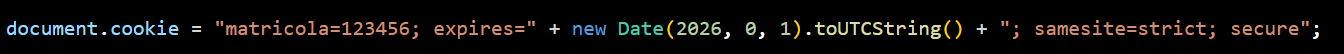
\includegraphics[width=15cm]{images/cookies/code_snippet.png}
  \caption{Esempio di creazione di un Cookie}
  \label{example_cookie:code_snippet}
\end{figure}
\begin{figure}[ht]
  \centering
  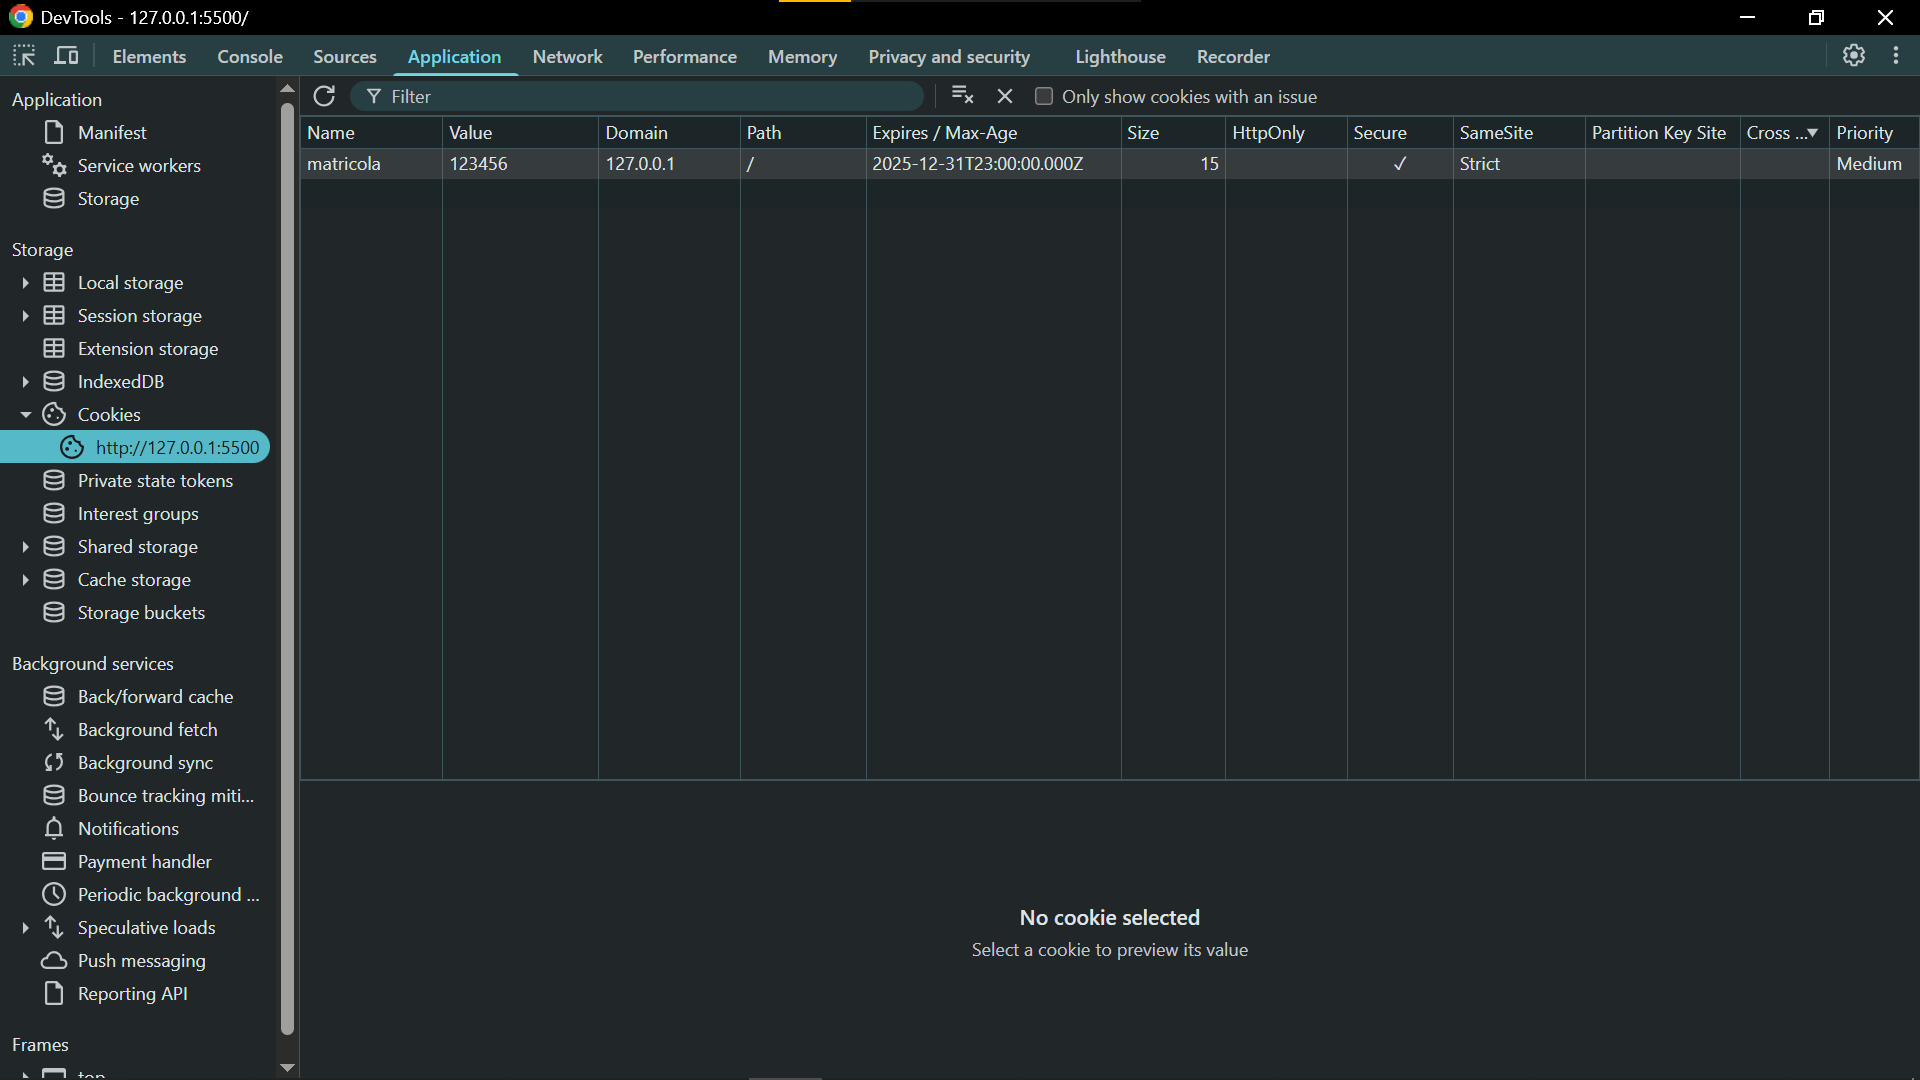
\includegraphics[height=7cm]{images/cookies/demonstration.png}
  \caption{Il Cookie creato prima}
  \label{example_cookie}
\end{figure}
Per quanto riguarda l'eliminazione dei Cookie, l'unica strategia disponibile è quella di sovrascrivere il Cookie con un altro avente scadenza già passata \cite{W3Schools:cookies}.\\
L'attributo \texttt{document.cookie} può anche essere acceduto in lettura: in tal caso si ottiene una lista delle sole coppie nome-valore di tutti i Cookie salvati in quel momento \cite{MDN_Web_docs:cookies}. Tutti gli altri parametri possono essere visualizzati solo da DevTools.

\section{Local Storage e Session Storage} %<-----MANCANO ESEMPI
\texttt{\textit{localStorage}} e \texttt{\textit{sessionStorage}} sono entrambi oggetti di tipo \texttt{Storage}: in quanto tali, essi permettono di salvare dati in memoria locale sottoforma di coppie chiave-valore (entrambe stringhe) \cite{MDN_Web_docs:storage_API}.\\
I due oggetti differscono per visibilità e durata: \texttt{localStorage} serve a contenere dati permanenti (cioè che rimangono in memoria indefinitamente, salvo esplicita rimozione da parte dell'utente o del programmatore) e condivisi fra le varie schede, per cui schede distinte del medesimo browser connesse allo stesso sito condividono lo stesso \texttt{localStorage} e, pertanto, modifiche apportate da una pagina sono visibili anche nell'altra pagina \cite{MDN_Web_docs:localStorage}. D'altro canto \texttt{sessionStorage} è progettato per contenere dati relativi alla singola sessione di navigazione: esso, quindi, non è condiviso fra schede e viene rimosso automaticamente alla chiusura della pagina (viene però conservato quando la pagina è ricaricata) \cite{MDN_Web_docs:sessionStorage}.\\
DevTools fornisce la possibilità di visualizzare \texttt{localStorage} e \texttt{sessionStorage} di una pagina: per browser Chromium-based è sufficiente cliccare su "\texttt{Application}" e poi "\texttt{Local Storage}" o "\texttt{Session Storage}" mentre per Firefox si deve cliccare su "\texttt{Storage}", quindi "\texttt{Local Storage}" o "\texttt{Session Storage}".
\subsection{implementazione}
Dato che \texttt{localStorage} e \texttt{sessionStorage} sono entrambi istanze di \texttt{Storage}, essi condividono la stessa API, composta dai metodi
\begin{itemize}
\item\texttt{setItem(key, value)}, che inserisce una nuova coppia chiave-valore in \texttt{Storage} se la chiave non è presente, altrimenti sostituisce il precedente valore a essa associato con il nuovo \cite{MDN_Web_docs:localStorage}.
\item\texttt{getItem(key)}, che restituisce il valore associato a \texttt{key} \cite{MDN_Web_docs:localStorage}.
\item\texttt{removeItem(key)}, che rimuove la coppia con chiave \texttt{key} \cite{MDN_Web_docs:localStorage}.
\item\texttt{clear()}, che svuota l'intero \texttt{Storage} \cite{MDN_Web_docs:localStorage}.
\item\texttt{key(n)}, che restituisce il nome della \texttt{n}-esima chiave \cite{MDN_Web_docs:localStorage}. 
\end{itemize}
È definito anche l'evento "\texttt{storage}", che viene lanciato quando il contenuto dello \texttt{Storage} subisce delle modifiche: questo evento può essere catturato da tutte le schede connesse allo \texttt{Storage} diverse dalla pagina che ha modificato il contenuto. Per ascoltare questo evento basta aggiungere un opportuno \texttt{event listener} all'oggetto \texttt{window} \cite{MDN_Web_docs:storage_API}.\\
\texttt{localStorage} e \texttt{sessionStorage} non sono disegnati per contenere una grande quantità di dati: un oggetto di tipo \texttt{Storage}, infatti, ha una capienza massima di 10MB. Se è necessario memorizzare grandi moli di dati bisogna ricorrere a \texttt{IndexedDB} \cite{MDN_Web_docs:IndexedDB_basic}.

\section{IndexedDB} %<---NON È PROGETTATO PER SERVER-SIDE
Gli \textit{\texttt{IndexedDB}} (\textit{Indexed database}) costituiscono un'altra strategia con cui le Web App possono immagazzinare dati nel Browser dell'utente. Un \texttt{IndexedDB} implementa un \textit{Object Oriented Database Management System} (\textit{OODBMS}) e, in quanto tale, memorizza coppie chiave-valore.\\
A differenza di \texttt{localStorage} e \texttt{sessionStorage}, \texttt{IndexedDB} non presenta limiti di spazio, inoltre chiavi e valori possono essere un qualunque oggetto, non per forza stringhe.\\
Mentre in un \textit{RDBMS} (\textit{Relational Database Management System}) i dati sono memorizzati come righe all'interno di una tabella, in un OODBMS essi sono salvati come oggetti all'interno di \textit{Object Store}: all'interno di un Object Store ciascun record sarà identificato da una \textit{chiave} univoca (come nei RDBMS), che può essere sfruttata per ottenere il riferiìmento al valore associato.\\
Oltre che con le chiavi, gli OODBMS possono essere interrogati anche attraverso \textit{indici}: un indice è un Object Store ausiliario che si riferisce a un altro Object Store, e che serve a effettuare ricerche su quest'ultimo. A titolo di esempio, si supponga di implementare un semplice database che registri i voti di un esame: esso è composto da un solo Object Store "\textit{exam}", in cui ogni record ha per chiave la matricola dello studente e per valore il suo voto. È ora possibile costruire un indice "\textit{grades}" che permette di effettuare ricerche in base ai voti (ad esempio cercare tutti gli studenti che hanno preso trenta e lode).\\
All'interno di un indice cisacun record ha valore che coincide con la chiave di un altro record all'interno dell'Object Store riferito; inoltre, ogni volta che il contenuto di quest'ultimo subisce una modifica, l'indice viene aggiornato automaticamente.\\
Quando si effettua una ricerca tramite indice, il risultato che viene restituito non è una lista di record bensì un \textit{cursore}, oggetto ausiliario negli OODBMS che permette di iterare fra record di un Object Store.\\
Gli indexed database applicano un modello basato su \textit{transazioni}, cioè una sequenza di operazioni che va a costituire un'unità logica di lavoro: qualunque modifica apportata al database deve essere eseguita entro una transazione. Le transazioni sono atomiche, ciò vuol dire che esse possono o essere completate nella loro interezza o non avere alcun effetto, dunque, se una delle operazioni della sequenza fallisce, è necessario annullare tutte le modifiche effettuate dalle precedenti operazioni. Inoltre, il fatto che le transazioni siano atomiche le rendono sicure nel caso in cui più finestre del browser tentino di accedere concorrentemente al database.\\
La indexedDB API presenta delle limitazioni, fra cui il fatto che è prpogettata per la gestione di un server solamente Client-Side, non sono forniti strumenti per la gestione Server-Side.\\
\subsection{Implementazione}
La IndexedDB API è principalmente asincrona, ciò vuol dire che la maggioranza delle operazioni sulla base di dati è eseguita per mezzo di \textit{richieste}: in javascript esse sono rappresentate mediante un oggetto di tipo \texttt{IDBRequest}, il quale presenta i metodi \texttt{onSuccess()} e \texttt{onError()} che permettono di definire delle callback functions da eseguire rispettivamente in caso di successo o errore.\\
È possibile inviare una richiesta di apertura della connessione con il database per mezzo della funzione \texttt{window.indexedDB.open()}, questa funzione richiede due parametri: il primo è il nome del database (che deve essere unico all'interno del dominio) e il secondo è la sua versione. Aprire un database con lo stesso nome di uno già esistente ma numero di versione maggiore viene interpretato come la richiesta di effettuare un aggiornamento sul database stesso. Per gli oggetti di tipo \texttt{IDBOpenDBRequest} (la richiesta restituita da \texttt{open()}), è presente anche il metodo \texttt{onupgradeneeded()} che definisce che funzione eseguire quando viene lanciato l'evento \texttt{upgradeneeded}.\\
\backmatter

\begingroup %------------------------------ BIBLIOGRAPHY
  \makeatletter
  \let\ps@plain\ps@empty
  \makeatother
  \bibliography{report}
  \addcontentsline{toc}{chapter}{Bibliografia}
  \bibliographystyle{ieeetr} % sort in order of appearance
\endgroup
\end{document} 